\documentclass[italian,12pt,a4paper,oneside,final]{report}
\usepackage[toc]{appendix}
\usepackage{listings}
\usepackage{graphicx}
\usepackage{biblatex} %Imports biblatex package
\usepackage[utf8]{inputenc}
\usepackage[italian]{babel}
\usepackage{csquotes}
\usepackage{hyperref}
\addbibresource{siotd.bib} %Import the bibliography file
\graphicspath{ {images/} }
\lstset{captionpos=b,showspaces=false,basicstyle=\ttfamily,showstringspaces=false,breaklines=true}
\renewcommand{\thesection}{\arabic{section}} % remove the \chapter counter from being printed with every \section
\renewcommand{\appendixtocname}{Appendice}
\renewcommand{\appendixpagename}{Appendice}
\hypersetup{
	colorlinks=true,
	linkcolor=,
	pdftitle={Marco Giunta - Progetto SIoTD},
	pdfauthor={Marco Giunta},
}

\title{\huge Smart Temperature Monitor\\[0.5em]
\large Relazione Progetto SIoTD24}
\date{Febbraio 2025}
\author{
Marco Giunta\thanks{Marco Giunta 147852 giunta.marco@spes.uniud.it}}

\begin{document}
% Generate title page
\maketitle

% Generate TOCs
\pagenumbering{arabic}
\tableofcontents

\newpage

\section{Introduzione}
Una delle sfide chiave del XXI secolo è l’adattamento ai cambiamenti climatici.
Per riuscire a limitare il riscaldamento globale è necessario impiegare l’energia in modo efficiente ed evitare gli sprechi: lasciare una finestra aperta in inverno o in estate vuol dire far raffreddare o riscaldare troppo una stanza, con conseguente spreco di energia per ripristinare la temperatura adeguata.
Dimenticarsi di spegnere il climatizzatore/riscaldamento la sera prima di andare via o durante il weekend, lasciare per molte ore una stanza vuota climatizzata più del necessario, sono situazioni che capitano spesso e contribuiscono ad aumentare lo spreco di energia.

Con questo progetto si vuole realizzare un prototipo a basso costo di un dispositivo \emph{smart} in grado di rilevare anomalie termiche all'interno di una stanza di un edificio pubblico, ad esempio un'università.

Il progetto ha come obiettivo il monitoraggio della temperatura della stanza in modo da rilevare valori oltre o sotto una certa soglia: le misure saranno salvate in un database e sarà possibile visualizzarle su una dashboard.
Se per un certo lasso di tempo all'interno quella stanza non c'è nessuno, il dispositivo sarà in grado di inviare un segnale di allarme al presidio tecnico del edificio, oppure attivare un attuatore per chiudere la finestra o il condizionatore.
Grazie ad un bot Telegram sarà possibile visualizzare la temperatura della stanza, modificare il valore della soglia del troppo caldo/freddo e recuperare l’informazione della presenza o meno di persone nella stanza.

Per raccogliere i dati è stato utilizzato il sistema di gestione di database InfluxDB\footfullcite{influxdb} mentre, per la parte di visualizzazione tramite dashboard, è stato utilizzato il software Grafana\footfullcite{grafana}.

Per l'installazione e configurazione del database InfluxDB e il software Grafana è stata utilizzata la tecnologia dei container.

\newpage

\section{Componenti}
Per la realizzazione del prototipo sono stati utilizzati questi componenti:

\begin{itemize}
\item Raspberry Pi 4 Model B, RAM 2GB 
\item Sensore di temperatura e umidità DHT22
\item Camera con sensore IMX219
\item LED e resistenze
\end{itemize}

\subsection{Schema elettrico}
\begin{figure}[h]
	\centering
	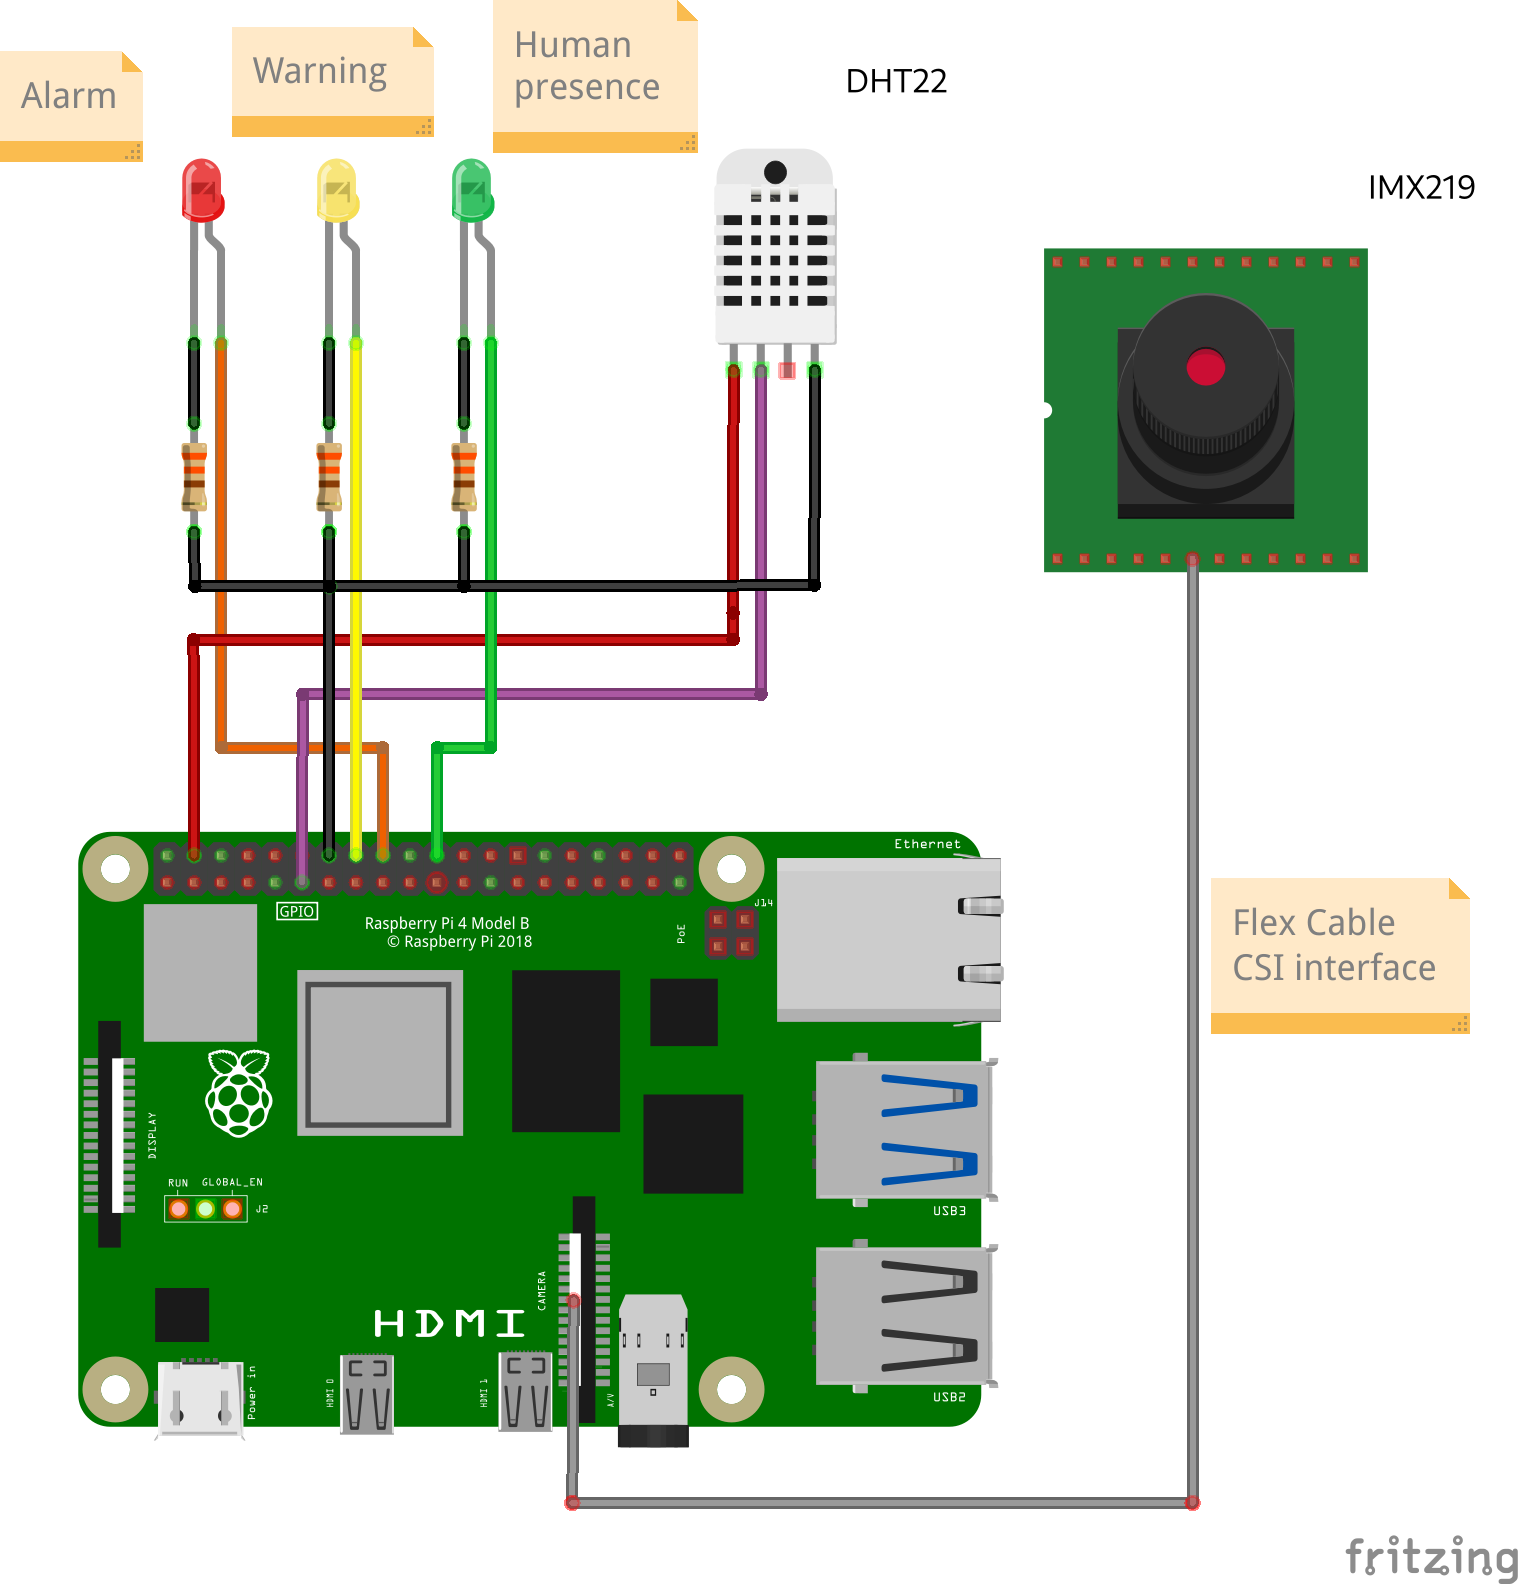
\includegraphics[scale=0.8]{rpi4_temp_sensor.png}
	\caption{Schema di collegamento}
	\label{fig:raspberry}
\end{figure}

\newpage

\subsection{Raspberry Pi 4 Model B}
La scheda Raspberry Pi 4b è un single-board computer che integra al suo interno un processore Broadcom BCM2711 quad-core Cortex-A72 (ARM v8) 64-bit,  2GB di memoria RAM, connessione cablata Gigabit Ethernet e wireless Wi-Fi 802.11b/g/n/ac.
Ci sono 40 pin: 12 sono di alimentazione (5V, 3.3V o GND) e 28 pin GPIO, configurabili come ingresso/uscita. 
Di questi, 2 pin sono dedicati alla comunicazione I2C, 5 a quella SPI, 2 possono essere usati come seriale (UART) e 4 sono pin PWM. 

\subsection{Sensore di temperatura e umidità}
Il sensore di temperatura e umidità utilizzato è il DHT22 AM2302: può funzionare a 5V e 3,3V.
Rispetto al sensore di temperatura DHT11, questo modulo consente una maggiore precisione nella misurazione della temperatura e dell'umidità.
Utilizzando un sensore di umidità capacitivo e un termistore, il sensore misura i dati dell'aria circostante e inoltra questi valori come segnale digitale al pin dati.

\subsection{Camera}
La videocamera utilizzata ha una risoluzione di 8MP e usa un sensore di immagine Sony IMX219.
È in grado di generare immagini statiche da 3280 x 2464 pixel e supporta anche video a 1080p30, 720p60 e 640x480p90.
Si collega al Raspberry Pi tramite l’interfaccia CSi standard dedicata.

\newpage

\section{Codice Python}
Il funzionamento dello \emph{Smart Temperature Monitor} è riassunto dal diagramma di flusso in figura~\ref{fig:flowchart}.
\begin{figure}[h]
	\centering
	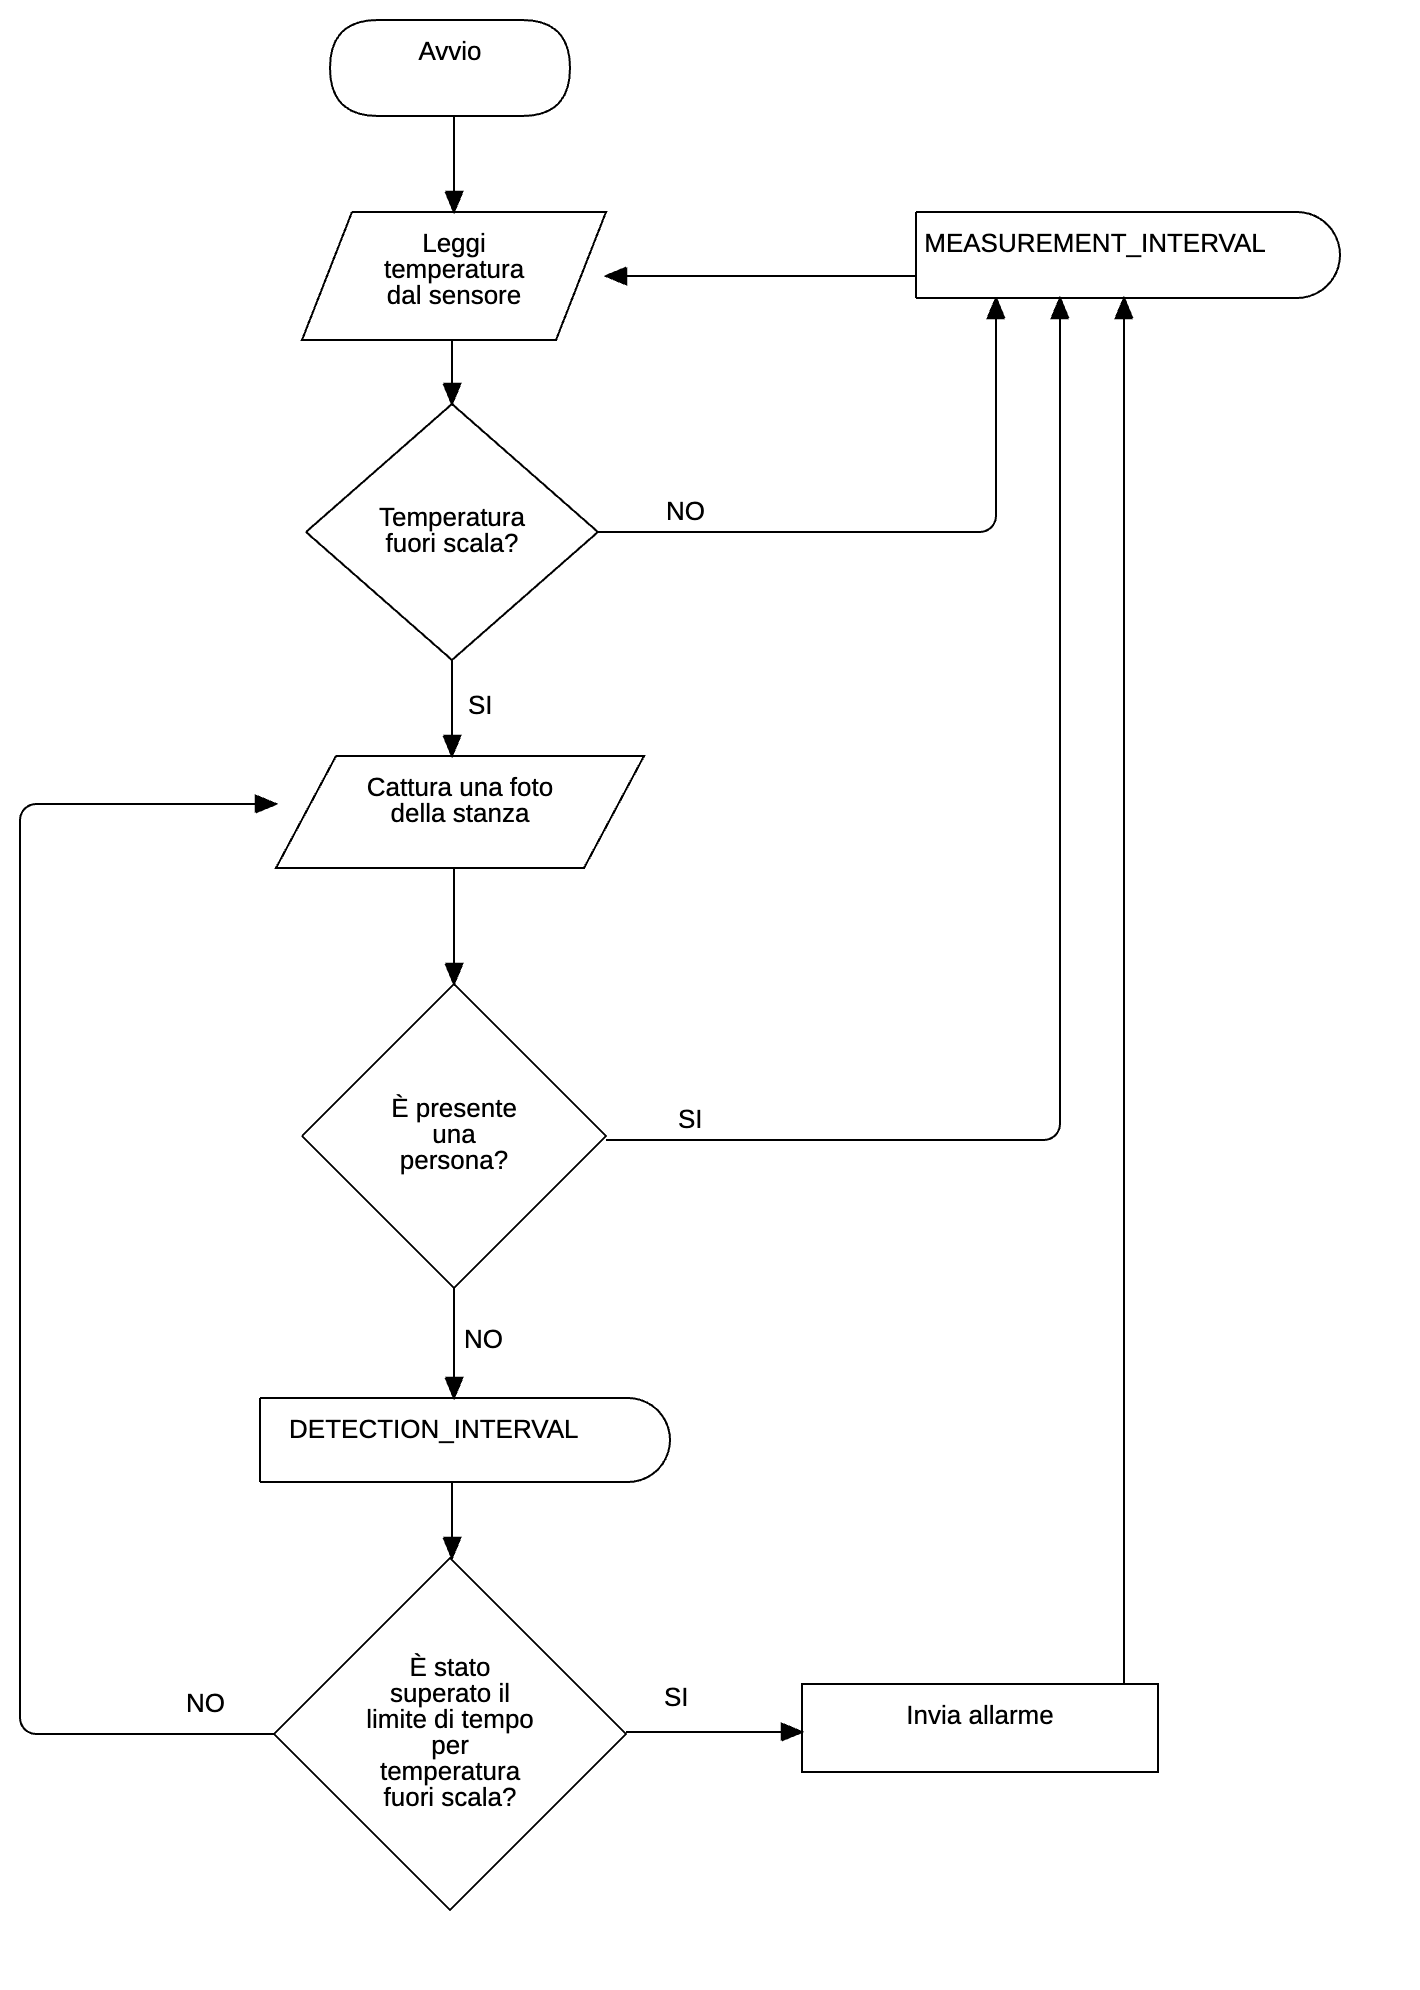
\includegraphics[scale=0.215]{flowchart.png}
	\caption{Diagramma di flusso semplificato}
	\label{fig:flowchart}
\end{figure}
Vediamo in dettaglio le diverse fasi.

\subsection{Lettura temperatura}
Per leggere dal sensore DHT22 i valori di temperatura e umidità è stata usata la libreria adafruit-circuitpython-dht\footfullcite{adafruit-dht}.
Durante la fase iniziale di progettazione è emersa una certa instabilità nelle letture, forse dovuta al sensore difettoso o di scarsa qualità.
Per evitare problemi con il resto del codice è stata inserita una procedura di reset in un blocco \textit{try..except}.

\subsection{Cattura di un immagine della stanza}
Il modulo camera utilizzato nel progetto non è il Camera Module 2 ma una versione compatibile con la scheda Jetson Nano: utilizza lo stesso sensore Sony IMX219 e lo stesso cablaggio.
Per far riconoscere questo modulo al sistema operativo Raspberry Pi OS è stato necessario modificare il file \textit{/boot/config.txt}, aggiungendo queste due impostazioni:
\begin{lstlisting}
camera_auto_detect=0
dtoverlay=imx219
\end{lstlisting}
Dopo la modifica, il modulo camera può essere utilizzato attraverso la libreria picamera2\footfullcite{picamera2}.

Durante l'inizializzazione della libreria, per migliorare l'immagine catturata dal modulo camera, è stato applicato un file di tuning per sensore NoIR, attivato l'auto-bilanciamento del bianco e scelta una risoluzione con un angolo di campo (FoV - field of view) pieno, in modo da utilizzare tutta la superfice del sensore per catturare l'immagine. 

\subsection{Rilevamento persone}
Per rilevare eventuali persone all'interno della stanza è stata utilizzata la libreria Ultralytics YOLO11\footfullcite{yolo11}.

Viste le ridotte risorse computazionali del Raspberry Pi, il modello YOLO11n è stato convertito in formato NCNN: in questo modo la libreria Ultralytics garantisce le migliori prestazioni su sistemi Embedded e dispositivi IoT.

Sulle immagini catturare dal modulo camera viene fatto il rilevamento \underline{solo} delle persone e, nel caso, l'immagine viene annotata.

\subsection{Invio allarme}
Per simulare l'invio di un allarme viene acceso un LED di colore rosso e viene inviato un messaggio ad un bot Telegram. 
Se il progetto dovesse trovare un utilizzo reale, è possibile modificare facilmente il codice per attivare un attuatore oppure inviare un messaggio a un broker MQTT\footfullcite{mqtt}.

\subsection{Bot Telegram}
Per interfacciarsi con lo \emph{Smart Temperature Monitor} è stato creato un bot Telegram.
Attraverso il bot è possibile modificare alcuni parametri del sistema, recuperare la temperatura della stanza e una foto della stessa in tempo reale.
I comandi disponibili sono:

\begin{itemize}
	\item[/picture] Si riceve una foto della stanza: se viene rilevata la presenza di persone, la foto sarà annotata.
	\item[/people] Restituisce il numero di persone presenti nella stanza.
	\item[/temperature] Si ottiene la temperatura attuale della stanza.
	\item[/maximum] È possibile modificare la soglia massima di temperatura.
	\item[/minimum] È possibile modificare la soglia minima di temperatura.
	\item[/offset] È possibile modificare il valore di temperatura rilavato.
\end{itemize}

\subsection{Invio dati al database}
Per il salvataggio dei dati viene utilizzato un database InfluxDB\footfullcite{influxdb}.
Ogni misurazione è \textit{taggata} con il numero di stanza, in modo da facilitare la creazione di una dashboard nel caso si utilizzino un numero elevato di \emph{smart monitor}.

\newpage
\section{Presentazione dei dati}
Per visualizzare i dati misurati dallo \emph{Smart Temperature Monitor} è stata realizzata una dashboard Grafana.
I valori rilevati dal sensore di temperatura vengono salvati all'interno di un database InfluxDB.
Tutti questi componenti software sono stati installati e configurati usando Docker.

\begin{figure}[h]
	\centering
	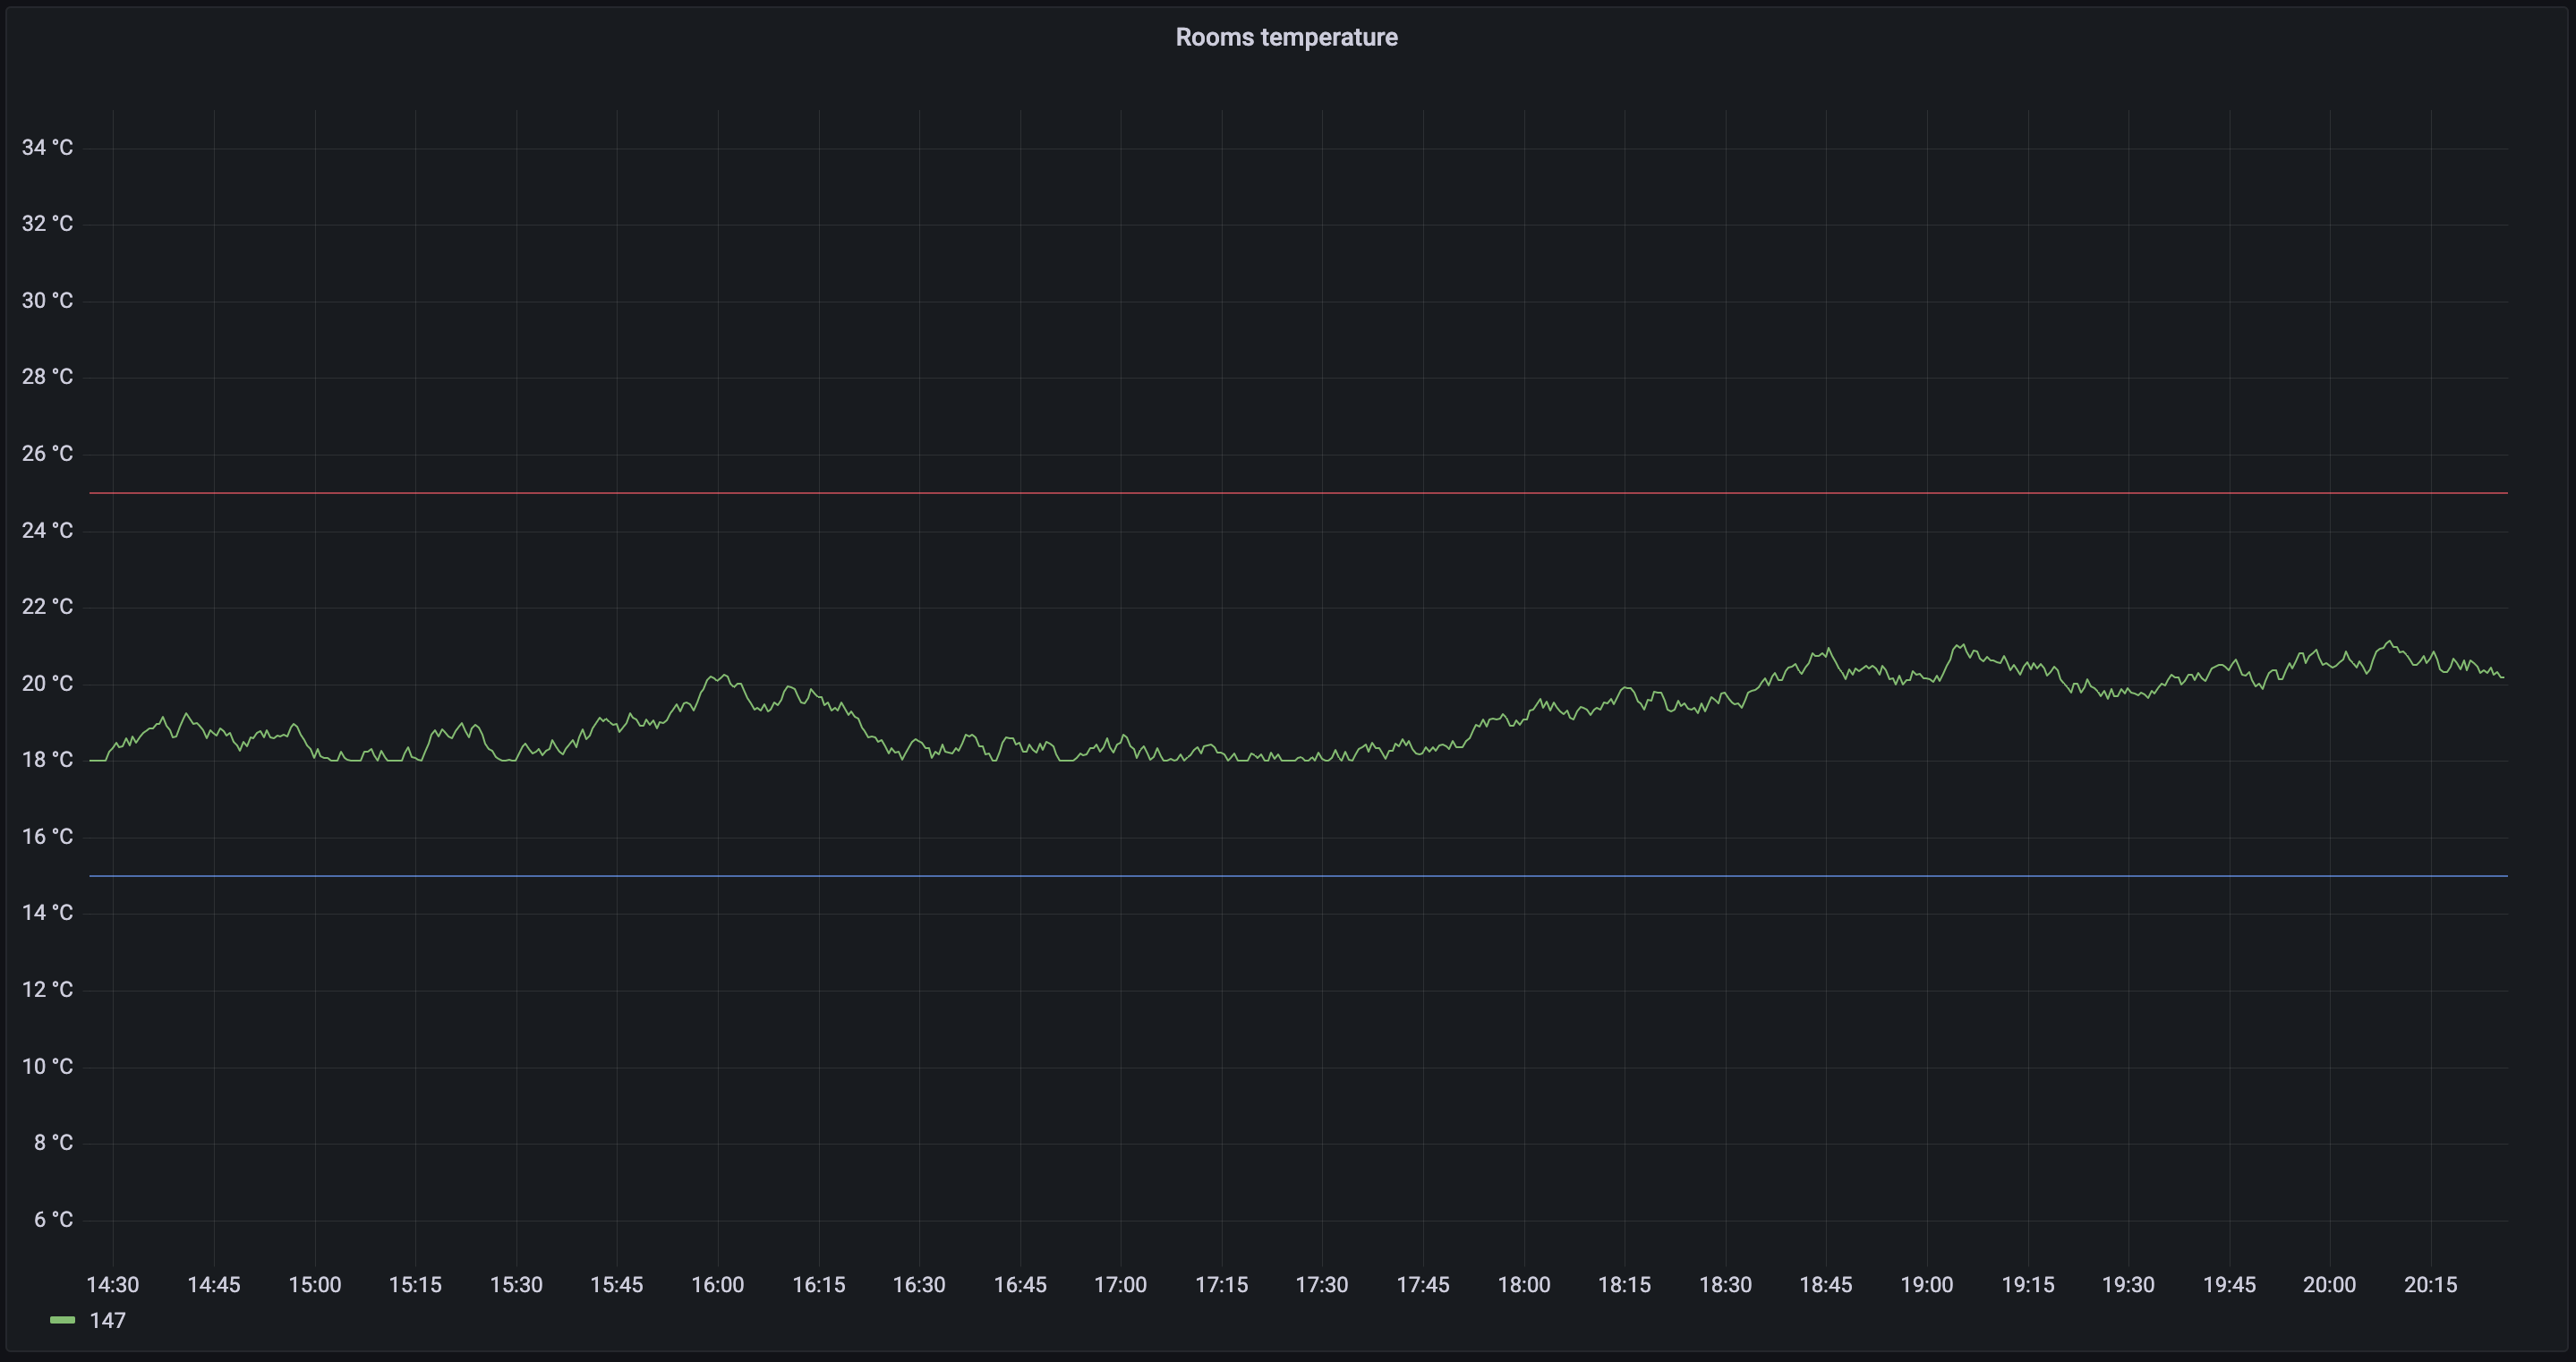
\includegraphics[width=1\textwidth]{grafana_room.png}
	\caption{Valori rilevati durante una giornata infrasettimanale}
	\label{fig:grafana_stanza}
\end{figure}

Nella figura~\ref{fig:grafana_stanza} si possono vedere i dati rilevati all'interno di una stanza che non presenta anomalie termiche.

\newpage

\section{Conclusioni}
Il prototipo realizzato ha raggiunto gli obiettivi previsti: è uno \textit{Smart Temperature Monitor}, realizzabile a basso costo, in grado di rilevare la presenza di persone nella stanza e inviare i dati tramite rete.
Anche se il sensore utilizzato nel progetto non è di tipo professionale, i valori rilevati sono abbastanza precisi e permettono una valutazione della temperatura reale di qualunque stanza.
Inoltre, nonostante le ridotte risorse computazionali del Raspberry Pi e la qualità del modulo camera, il rilevamento delle persone si è dimostrato coerente.

Data la semplicità e il basso costo di realizzazione, il progetto può essere utilizzato per monitorare la temperatura di tutte le stanze all'interno di un edificio.
La possibilità di visualizzare le temperature in tempo reale, tramite una dashboard Grafana, e il rilevamento delle persone sono un aiuto importante nella valutazione delle azioni da intraprendere per ridurre i consumi energetici, identificando le stanze vuote con temperature anomale.

\appendices
\noindent{\huge\bfseries APPENDICE\par}

\section{Docker Compose}
\begin{lstlisting}[caption=docker-compose.yaml]
services:
  influxdb:
    image: influxdb:1.8
    environment:
      - TZ=Europe/Rome
      - INFLUXDB_DB=defaultdb
      - INFLUXDB_ADMIN_ENABLED=true
      - INFLUXDB_ADMIN_USER=admin
      - INFLUXDB_ADMIN_PASSWORD=adminpass
      - INFLUXDB_USER=user
      - INFLUXDB_USER_PASSWORD=userpass
    ports:
      - "8086:8086"
    networks:
      - iot
    volumes:
      - influxdb:/var/lib/influxdb
    restart: always

  grafana:
    image: grafana/grafana:8.4.6-ubuntu
    ports:
      - "3000:3000"
    networks:
      - iot
    volumes:
      - grafana:/var/lib/grafana
    depends_on:
      - influxdb
    restart: always

  networks:
    iot:

  volumes:
    influxdb:
    grafana:
\end{lstlisting}

\end{document}
